% ============================================================
% GitSyntropy — WorldSUAS 2026 IEEE Conference Paper
% "Predicting Software Team Compatibility via Behavioral
%  Telemetry and Adaptive Psychometric Profiling"
%
% Author: 1mystic (IIT Madras, 23f2004201@ds.study.iitm.ac.in)
% Template: IEEEtran conference, double-column, 10pt
% ============================================================
\documentclass[conference]{IEEEtran}
\IEEEoverridecommandlockouts

\usepackage{cite}
\usepackage{amsmath,amssymb,amsfonts}
\usepackage{algorithmic}
\usepackage{algorithm}
\usepackage{graphicx}
\graphicspath{{figures/}{./}}
\usepackage{textcomp}
\usepackage{xcolor}
\usepackage{booktabs}
\usepackage{url}
\usepackage{microtype}
\usepackage{balance}
\usepackage{array}
\usepackage{multirow}

\def\BibTeX{{\rm B\kern-.05em{\sc i\kern-.025em b}\kern-.08em
    T\kern-.1667em\lower.7ex\hbox{E}\kern-.125emX}}

\renewcommand{\algorithmicrequire}{\textbf{Input:}}
\renewcommand{\algorithmicensure}{\textbf{Output:}}

% Slightly more breathing room between paragraphs
\setlength{\parskip}{0.25ex}

\begin{document}

% ============================================================
\title{Estimating Software Team Compatibility via Behavioral
Telemetry and Adaptive Psychometric Profiling}

\author{
  \IEEEauthorblockN{Atharv Khare}
  \IEEEauthorblockA{
    \textit{Department of Data Science and Artificial Intelligence}\\
    \textit{Indian Institute of Technology Madras}\\
    Chennai, India\\
    23f2004201@ds.study.iitm.ac.in
  }
}

\maketitle

% ============================================================
\begin{abstract}
Estimating software team friction before it manifests in missed
deadlines or degraded code quality remains an open problem in
empirical software engineering.  Existing approaches rely either on
static self-report personality instruments, which lack grounding in
observed work behavior, or on activity dashboards that report metrics
without producing actionable compatibility signals.  We present
\textit{GitSyntropy}, a multi-agent system that derives pairwise team
compatibility scores from two complementary signal streams: behavioral
telemetry extracted from GitHub commit and pull-request history, and
responses to an eight-item Computerized Adaptive Testing (CAT)
assessment.  The system applies K-Means clustering in circular
coordinate space to classify developer chronotypes from commit
timestamp distributions, fuses these signals with a weighted
eight-dimensional scoring model (maximum 36~points), and uses Monte
Carlo simulation to estimate the potential impact of candidate
profiles on team compatibility.  Evaluated on 46 real GitHub developer profiles
(10,886 commits), the chronotype classifier achieves a macro
F\textsubscript{1} of 0.860 (owl: 0.927, lark: 0.923) with 75\,\%
exact cross-modal agreement between GitHub and Stack~Overflow
activity-time labels ($n{=}20$).  The CAT algorithm guarantees early
stopping after five questions due to the weight-ordered design, with
a mean of 5.0 questions (37.5\,\%
reduction, $r{=}0.965$ score fidelity), and Monte Carlo variance
drops $3.6{\times}$ from 100 to 1,000 iterations.
Chronotype-aligned pairs score 35.74/36 versus 24.82/36 for
mismatched pairs ($p < 0.001$, Cohen's $d = 3.71$).
These results primarily reflect internal model behavior and require further validation against real-world team performance outcomes.
\end{abstract}

\begin{IEEEkeywords}
behavioral analytics, chronotype detection, team compatibility,
computerized adaptive testing, Monte Carlo simulation,
software engineering telemetry
\end{IEEEkeywords}

% ============================================================
\section{Introduction}
% ============================================================

Software team effectiveness depends not only on individual technical
skill but substantially on behavioral alignment: shared work rhythms,
compatible communication styles, and complementary decision-making
approaches.  Conway's law~\cite{herbsleb1999} established that the
communication structures of an organization are reflected in the
architecture of the software it produces.  More recent empirical
work shows that team composition and behavioral alignment predict
delivery outcomes as strongly as technical competence
alone~\cite{tamburri2019}.  Rosen et al.~\cite{rosen2011} identified
behavioral coordination---the sequencing and timing of interdependent
actions---as the primary observable marker of team adaptability,
with schedule misalignment directly degrading coordination capacity.
Teams that fail to deliver on schedule or produce defect-heavy
software frequently exhibit patterns of chronotype mismatch,
conflicting communication densities, and unresolved leadership
ambiguity~\cite{catolino2019}.  The cost of misalignment grows as
organizations scale distributed and hybrid teams, where asynchronous
handoffs amplify even modest schedule incompatibility into multi-day
integration delays.  In agile software teams specifically,
Bhuvaneswari et al.~\cite{bhuvaneswari2025} found that balanced
psychometric diversity significantly improves sprint efficiency and
reduces burnout risk---but existing tooling lacks the granularity
to detect these imbalances at the dyadic level before they manifest
in sprint retrospectives.

Current tools for team assessment occupy two inadequate positions.
\textit{Static psychometric instruments}---Myers-Briggs Type
Indicator (MBTI)~\cite{myers1943} and DiSC~\cite{marston1928}---rely
entirely on self-report and produce a single-point-in-time label
disconnected from observed work behavior; their test-retest
reliability and predictive validity for team performance have been
questioned~\cite{pittenger1993, halfhill2005}.  Approximately
50\,\% of MBTI respondents receive a different type label when
re-administered four weeks later.  \textit{Activity dashboards}
(GitHub Insights, Jira Analytics, Pluralsight Flow) capture
behavioral signals but present raw metrics without translating them
into actionable compatibility scores~\cite{dingsoyr2012}.  No
published system combines behavioral telemetry from version control
with adaptive psychometric profiling to produce a pairwise
compatibility score.

We present \textit{GitSyntropy}, a system that addresses this gap
by integrating two independently observable signal streams.  The
first derives chronotype labels and collaboration metrics from the
public commit and pull-request history available in GitHub---an
approach that requires no active participation from developers
beyond their existing work.  The second administers a compact,
adaptive eight-item psychometric instrument that terminates early
once sufficient high-weight dimensions have been answered, reducing
respondent burden by 37.5\,\% without sacrificing score fidelity.
These signals are fused in a weighted eight-dimensional compatibility
engine, and a Monte Carlo simulator identifies the optimal candidate
hire profile for a given team.  A LangGraph multi-agent pipeline
orchestrates the full workflow, and Anthropic Claude (Sonnet model) synthesizes
the scores into a streaming narrative report.

\medskip
\noindent The contributions of this work are:
\begin{enumerate}
  \item A \textbf{circular-coordinate K-Means algorithm} for
    chronotype classification from VCS commit timestamps that
    correctly handles the midnight hour boundary via unit-circle
    projection.
  \item A \textbf{weighted eight-dimensional compatibility engine}
    (maximum 36 points) with confidence-aware neutral imputation
    for missing psychometric data.
  \item A \textbf{greedy information-maximizing CAT algorithm} that
    achieves early stopping at a mean of 5.0 out of 8 questions
    across all $5^8 = 390{,}625$ response permutations
    ($r = 0.965$ with full-length scores).
  \item A \textbf{Monte Carlo candidate simulation} that produces
    an optimal hire profile and improvement distribution over
    1,000 deterministic iterations.
  \item An \textbf{open-source full-stack implementation} with a
    LangGraph DAG pipeline, WebSocket-streamed LLM synthesis, and
    empirical validation on 46 real GitHub developer profiles.
\end{enumerate}

\medskip
The remainder of this paper is organized as follows.
Section~\ref{sec:background} provides scientific and historical
background.  Section~\ref{sec:related} surveys related work and
existing tools.  Section~\ref{sec:design} describes the system
design and algorithms.  Section~\ref{sec:eval} presents
experimental evaluation.  Section~\ref{sec:discuss} discusses
limitations and future directions.  Section~\ref{sec:conclusion}
concludes.

% ============================================================
\section{Background}
\label{sec:background}
% ============================================================

\subsection{Software Team Behavioral Dynamics}

Software engineering is increasingly a team-centered discipline.
Herbsleb and Grinter~\cite{herbsleb1999} showed that
communication-structure gaps within organizations translate directly
into integration failures in code.  Tamburri et al.~\cite{tamburri2019}
extended this into the notion of \textit{software organizational
debt}: the accumulated cost of suboptimal team structure, covering
human factors such as knowledge silos, chronotype misalignment, and
decision-style conflicts.  Catolino et al.~\cite{catolino2019}
operationalized team-level dysfunction as ``community smells''---
recurring patterns such as radio silence between subgroups or
over-reliance on a single contributor---and correlated their
presence with higher defect rates.

Work-hour misalignment is a particularly consequential source of
friction in distributed and hybrid teams.  Holmstr\"{o}m et
al.~\cite{holmstrom2006} studied globally distributed agile teams
and found that a four-hour overlap window was the minimum viable
synchronous contact for effective sprint coordination.  Below this
threshold, teams defaulted to asynchronous communication patterns
that introduced multi-day feedback delays in code review cycles.

\subsection{Chronotype Science and Measurement}

A developer's \textit{chronotype}---the biological tendency toward
morning, intermediate, or evening activity---is a stable
individual-difference variable with a heritability estimate of
approximately 50\,\%~\cite{roenneberg2003}.  Horne and
\"{O}stberg~\cite{horne1976} introduced the Morningness-Eveningness
Questionnaire (MEQ), a 19-item self-report instrument that remains
the gold standard for chronotype measurement.  Adan and
Almirall~\cite{adan1991} validated a five-item reduced version
(rMEQ, $r = 0.97$ with full MEQ) suitable for large-scale online
distribution.  The Munich Chronotype Questionnaire
(MCTQ)~\cite{roenneberg2003} takes an alternative approach, inferring
chronotype from self-reported sleep timing on free days.

Chronotype affects more than scheduling convenience.  Gunia et
al.~\cite{gunia2014} showed that self-regulatory capacity is
chronotype-dependent: morning types exhibit impaired ethical
reasoning in the evening and vice versa.  At the team level,
chronotype mismatch limits the hours during which high-quality
synchronous decision-making is possible and forces low-alertness
individuals to attend critical meetings outside their optimal
performance window.

The statistical challenge in measuring chronotype from timestamp
data is that clock time is \textit{circular}: hours 0 and 23 are
adjacent, not 23 units apart.  Fisher~\cite{fisher1993} provides the
formal framework for circular statistics, including the mean direction
and circular variance.  A naive arithmetic mean of hours (e.g.,
averaging 23 and 1 to get 12:00) produces a nonsensical result;
a circular mean correctly returns 00:00.
Intuitively, time is treated like a clock face, so 23:00 and 01:00
are close rather than far apart.

\subsection{The Ashtakoot Weight Structure}

We adopt a monotonic integer weighting scheme (1--8) as a structured
design prior for compatibility scoring.  The specific vector used in
GitSyntropy---$\{1,2,3,4,5,6,7,8\}$ summing to 36---is loosely adapted
from the \textit{Ashtakoot} (Sanskrit: ``eight attributes'') scheme,
documented in the classical Indian astronomical treatise
\textit{Brihat Parashara Hora Shastra} (attributed to Parashara Muni,
c.\ 600--800~CE).  We borrow only the idea of eight differentially
weighted dimensions and the aggregate ceiling of 36 points.

\textbf{What GitSyntropy borrows:} only the integer weight vector
$(1,2,3,4,5,6,7,8)$ and the aggregate ceiling of 36.  The
astronomical inputs---lunar constellation positions (\textit{nakshatras}),
planetary lords (\textit{grahas})---are discarded entirely.

\textbf{Scientific motivation for the mapping:} the weight ordering
encodes a design prior that higher-weighted attributes are more
consequential to long-term compatibility.  We map the original
kootas to software team dimensions based on face validity and
supporting empirical evidence:

\begin{itemize}
  \item \textbf{Nadi (8) $\to$ Chronotype Sync.}  Nadi concerns
    physiological ``channel'' compatibility in the original
    system---the most fundamental biological-level match.
    Chronotype alignment is the directly observable schedule-level
    equivalent, and schedule misalignment is the most widely
    documented source of distributed-team friction~\cite{holmstrom2006}.
  \item \textbf{Bhakoot (7) $\to$ Stress Response.}  Bhakoot
    relates to prosperity and the capacity to sustain the relationship
    under adversity---mapped to how team members handle deadline
    pressure, which determines team longevity under sprint stress.
  \item \textbf{Gana (6) $\to$ Risk Tolerance.}  Gana classifies
    temperament into three categories (divine, human, demonic) that
    broadly map to risk appetite: bold experimentation versus
    methodical caution.
  \item \textbf{Graha Maitri (5) $\to$ Decision Style.}  Planetary
    friendship in the original system determines cognitive
    compatibility---mapped here to data-driven versus intuitive
    decision-making preference.
  \item \textbf{Yoni (4) $\to$ Work Style,} Tara (3) $\to$ Team
    Resilience, Vashya (2) $\to$ Leadership Orientation,
    Varna (1) $\to$ Innovation Drive.  These follow decreasing
    operational impact on day-to-day team functioning.
\end{itemize}

This borrowing is analogous to adopting Fibonacci spacing for agile
story-point estimation~\cite{wainer2000}: the sequence is chosen for
its structural properties (increasing gaps that force meaningful
distinctions between estimates), not for the underlying mathematics.
The weight-structure hypothesis will be replaced by empirically
calibrated factor loadings in future work.

% ============================================================
\section{Related Work}
\label{sec:related}
% ============================================================

\subsection{Mining Software Repositories for Behavioral Signals}

The Mining Software Repositories (MSR) community has established
that a developer's public GitHub history is a rich behavioral
signal.  Kalliamvakou et al.~\cite{kalliamvakou2014} catalogued
the systematic biases in GitHub data (pull-based vs.\ push-based
workflows, bot accounts, mirror repositories) that must be
mitigated before drawing conclusions.  Bird et al.~\cite{bird2009}
showed that commit network topology---who reviews whose code---
predicts post-release defect density, demonstrating that behavioral
relationships encoded in VCS history have measurable quality
consequences.

Claes et al.~\cite{claes2018} focused specifically on work-time
distributions, analyzing 1,000 GitHub developer commit histories and
finding that approximately 16\,\% of developers commit primarily
during late-night hours (22:00--05:00 UTC) and 9\,\% during early
morning (05:00--09:00 UTC).  Their analysis used naive histogram peak
detection, which misclassifies developers whose primary activity
straddles midnight.  Our circular-coordinate K-Means resolves this
by projecting hours to the unit circle before clustering, where
hours 0 and 23 have Euclidean distance $2\sin(\pi/24) \approx 0.26$
rather than 23 on the linear scale.

\subsection{Chronotype Inference from Digital Traces}

Several studies have inferred chronotype from passively collected
digital traces without requiring explicit self-report.
Aledavood et al.\ (2015) used smartphone usage logs (call and SMS
timestamps) to classify early and late chronotypes, achieving
agreement with MEQ in 78\,\% of cases.  Walch et al.\ (2016)
inferred chronotype from wearable accelerometer data (sleep onset
and offset timing).  Our approach applies the same passive-trace
philosophy to version control systems: the developer's commit
timestamps are the behavioral log, and the circular K-Means
algorithm is the inference engine.

\subsection{Psychometric Profiling for Software Teams}

The Big Five personality model (OCEAN)~\cite{mccrae1987} is the
dominant scientifically validated framework for individual
differences.  Several studies have correlated Big Five traits with
software engineering outcomes: conscientiousness predicts code
quality, openness predicts adoption of new technologies, and
agreeableness predicts code review collaboration~\cite{halfhill2005}.
However, the Big Five was not designed for team compatibility
prediction, and its broad trait dimensions require a mapping
step before they can produce pairwise scores.

Rosen et al.~\cite{rosen2011} provided a comprehensive process model
of team adaptation, identifying behavioral markers across four
phases: situation assessment, plan formulation, plan execution, and
team learning.  Their framework establishes that behavioral
\emph{coordination}---the sequencing and timing of interdependent
actions---is the single most observable indicator of team
adaptability.  This motivates GitSyntropy's Chronotype Sync
dimension: schedule misalignment directly degrades coordination
capacity by reducing the overlap window in which synchronous work
is possible.  Rosen et al.\ also highlight psychological safety as
a cross-cutting enabler, a construct that maps onto GitSyntropy's
Communication Density and Conflict Resolution dimensions.

Bhuvaneswari et al.~\cite{bhuvaneswari2025} introduced a
data-driven psychometric intelligence framework for agile software
teams, integrating Big Five Inventory (BFI-44) and Emotional
Intelligence Scale assessments with sprint-velocity and code-commit
behavioral logs across 120 professionals in 18 agile teams.  Their
findings show that balanced psychometric diversity---combining
analytical thinkers, conscientious executors, and emotionally stable
communicators---produces measurable improvements in sprint efficiency
and burnout resilience.  GitSyntropy operationalizes a complementary
hypothesis at the pairwise level: rather than optimizing aggregate
team composition, it scores each developer dyad across eight
dimensions, allowing managers to identify specific friction points
rather than composite team health indices.

MBTI~\cite{myers1943} assigns individuals to one of 16 types using
four forced dichotomies (E/I, S/N, T/F, J/P).  Pittenger~\cite{pittenger1993}
showed that approximately 50\,\% of respondents receive a different
type on re-administration four weeks later, and that MBTI
scores show weak or inconsistent correlations with job performance.
DiSC~\cite{marston1928} maps individuals to four behavioral quadrants
(Dominance, Influence, Steadiness, Conscientiousness) but lacks
peer-reviewed normative data for software engineering populations.

Belbin's team-role model~\cite{belbin1981} takes a more empirically
grounded approach: it identifies nine complementary behavioral roles
(Coordinator, Shaper, Plant, Resource Investigator, Monitor-Evaluator,
Teamworker, Implementer, Completer-Finisher, Specialist) and shows
that teams with balanced role coverage outperform homogeneous teams.
GitSyntropy's eight behavioral dimensions are philosophically closer
to Belbin than to MBTI: they target collaboration-relevant tendencies
rather than abstract personality traits.

The design and validation of psychometric instruments for software
engineering contexts requires careful adherence to psychometric
methodology.  Graziotin et al.~\cite{graziotin2021} provide a
comprehensive methodological framework for psychometrics in
behavioral software engineering, warning that instrument
modifications---including item reordering or truncation---can
destroy validity and reliability properties.  Consistent with their
guidelines, GitSyntropy's eight-item assessment preserves item
integrity while using a greedy weight-maximization early-stop
strategy (rather than item modification) to reduce assessment
burden.

\subsection{Computerized Adaptive Testing}

Classical CAT systems use Item Response Theory (IRT)---typically the
three-parameter logistic (3PL) model---to select the next assessment
item that provides the maximum information at the current latent
ability estimate~\cite{vanderlinden2000}.  Wainer et al.~\cite{wainer2000}
demonstrated that adaptive administration reduces test length by
50\,\% with minimal accuracy loss across a broad range of ability
levels.  For fixed-bank instruments with fewer than 16 items, full
IRT model fitting is impractical due to small item-parameter
estimation samples.  Greedy weight-maximization preserves the key
adaptive property (high-information items first) without requiring
parameter estimation, making it suitable for the eight-item
instrument used here.

\subsection{Team Composition Optimization}

Computational team formation has been treated as a combinatorial
optimization problem with skill coverage as the objective.
Fitzpatrick and Askin~\cite{fitzpatrick2005} formulated multi-skill
team formation as an integer program.  Lappas et al.~\cite{lappas2009}
framed it as a graph problem over social networks, minimizing
communication cost while covering a required skill set.  Both
frameworks treat team members as static skill vectors, without
incorporating behavioral compatibility signals.  Monte Carlo
search for candidate-impact optimization in the behavioral compatibility
space, as implemented in GitSyntropy, is---to our
knowledge---not previously described in the literature.

Closest to GitSyntropy's hire-simulation module is the
Trust--Personality Fit Matrix introduced by Maiti et al.~\cite{maiti2025},
which maps Big Five psychometric profiles to recommended operational
roles via a weighted Trust Calibration Index (TCI):
$\text{TCI} = \omega_1 \cdot \text{Openness} +
\omega_2 \cdot \text{Conscientiousness} -
\omega_3 \cdot \text{Neuroticism} + \omega_4 \cdot
\text{Emotional Stability}$.  Their TPMAP framework shows that
matching human operators to roles by psychometric profile reduces
trust mis-calibration in human-AI teams---a finding that supports
the feasibility of the analogous matching operation in GitSyntropy's
Monte Carlo candidate simulator.  The key structural difference is
scope: TPMAP optimizes individual-to-role assignment in a single
hiring decision, whereas GitSyntropy's simulator optimizes the
marginal improvement to the \emph{team-level} mean pairwise
compatibility score across all existing team members simultaneously.

The consequences of team composition on resilience under adversity
are documented empirically by Varaj\~{a}o et al.~\cite{varajao2021},
who used Structural Equation Modeling across information-systems
projects to show that Trust \& Solidarity, Commitment, and Skills
\& Behaviors are the primary determinants of project team resilience.
Their finding that two or more individually resilient people do not
necessarily constitute a resilient team provides theoretical
grounding for GitSyntropy's pairwise compatibility framing: team
resilience is an \emph{emergent} property of member interactions,
not a simple aggregate of individual traits.  GitSyntropy's Stress
Response and Team Resilience dimensions (weights 7 and 3,
respectively) are designed to capture precisely these interaction
patterns.  Grimm et al.~\cite{grimm2023} further corroborate this at
the dynamical-systems level, showing that team resilience is best
measured as the speed of system reorganization following a
perturbation---a metric that depends on prior coordination quality,
which our compatibility score is designed to predict ante hoc.

\subsection{Existing Commercial and Research Tools}

Table~\ref{tab:tools} summarizes the landscape of existing tools
and their coverage relative to GitSyntropy's feature set.
\textbf{15Five} and \textbf{Lattice} are continuous performance
management platforms that collect engagement survey responses and
display aggregate team health metrics; they produce no
pairwise compatibility scores and do not access VCS data.
\textbf{Pluralsight Flow} (formerly GitPrime) and \textbf{LinearB}
analyze commit patterns for engineering productivity metrics
(throughput, cycle time, PR review depth) but treat VCS data as
a workflow signal rather than a behavioral fingerprint.
\textbf{Haystack} similarly provides PR-cycle analytics without
behavioral profiling.  \textbf{Crystal Knows} predicts communication
style from LinkedIn text via natural language processing, relying
on public prose rather than behavioral telemetry; it produces
individual style labels rather than pairwise compatibility scores.
None of these tools combines commit-derived chronotype inference,
adaptive psychometric assessment, and candidate-impact simulation in a
unified pipeline.

\begin{table}[t]
\caption{Comparison of Team Analytics Tools}
\label{tab:tools}
\centering
\footnotesize
\setlength{\tabcolsep}{4pt}
\begin{tabular}{lcccc}
\toprule
Tool & VCS & Psychometric & Compatibility & Hire Sim. \\
\midrule
15Five / Lattice      & \texttimes & \checkmark & \texttimes & \texttimes \\
Pluralsight Flow      & \checkmark & \texttimes & \texttimes & \texttimes \\
LinearB / Haystack    & \checkmark & \texttimes & \texttimes & \texttimes \\
Crystal Knows         & \texttimes & \checkmark & Partial & \texttimes \\
\textbf{GitSyntropy}  & \checkmark & \checkmark & \checkmark & \checkmark \\
\bottomrule
\end{tabular}
\end{table}

% ============================================================
\section{System Design}
\label{sec:design}
% ============================================================

\subsection{Architecture Overview}

GitSyntropy operates as a five-stage pipeline executed by a LangGraph
directed acyclic graph (DAG) of asynchronous agent nodes
(Fig.~\ref{fig:arch}).  Each node receives and returns a typed
\texttt{OrchestratorState} TypedDict; LangGraph handles edge
routing, error propagation, and state checkpointing.  The pipeline
is triggered by a WebSocket connection from the client and emits
progress events at each stage boundary.

\begin{enumerate}
  \item \textit{GitHub Analyst:} fetches commit timestamps, pull
    requests, and collaboration metrics; runs circular K-Means
    chronotype classification.
  \item \textit{Psychometric Profiler:} administers the CAT
    assessment interactively over WebSocket and maps Likert responses
    to eight dimension scores.
  \item \textit{Compatibility Engine:} computes pairwise weighted
    similarity across all eight dimensions for each team member pair.
  \item \textit{Monte Carlo Simulator} (optional, triggered by
    \texttt{include\_candidates=True}): searches for the optimal
    hire profile given the current team composition.
  \item \textit{Synthesis Agent:} builds a structured prompt from
    the scores and streams a narrative compatibility report token
    by token via the Anthropic streaming API.
\end{enumerate}

The backend is implemented in FastAPI (async Python 3.12) with
SQLAlchemy + asyncpg and Supabase (PostgreSQL) for persistent
storage of profiles and team histories.  The frontend is built with
Astro~4 + React and Recharts for interactive score visualizations.
Results stream token-by-token over WebSocket to minimize perceived
latency.

\begin{figure}[t]
  \centering
  
\includegraphics[width=\columnwidth]{fig1_architecture}
  \caption{GitSyntropy pipeline: five async LangGraph nodes from
    GitHub data ingestion to streamed LLM narrative synthesis.
    Dashed brace denotes the LangGraph DAG boundary.}
  \label{fig:arch}
\end{figure}

\subsection{GitHub Data Ingestion}

For each developer, three async calls run concurrently within the
GitHub Analyst node:

\begin{enumerate}
  \item \textbf{Commit timestamps:} iterates over user-owned
    repositories and fetches commits authored by the target
    username within a 90-day lookback window, collecting the
    UTC hour of each commit.
  \item \textbf{Pull-request metrics:} counts PRs created by
    the developer and computes an after-hours ratio
    (fraction created between 20:00 and 07:00~UTC).
  \item \textbf{Collaboration index:} counts PR review comments
    authored by the developer (each comment contributes~2 points,
    capped at 100), producing a proxy for review engagement.
\end{enumerate}

Timestamps are extracted as UTC integers via
\texttt{datetime.fromisoformat(ts.replace("Z", "+00:00")).hour}
to avoid locale-dependent timezone interpretation.  Bot accounts
are excluded by matching display names against common CI/CD agent
patterns (\texttt{github-actions}, \texttt{dependabot}, etc.).
The GitHub REST API rate budget is approximately 5,000 requests
per hour per authenticated token; a full single-developer analysis
consumes 15--30 requests.

\subsection{Chronotype Classification}

Raw commit hours are noisy: a developer working across midnight
produces hour values near~0 and~23 that appear 23~units apart on a
linear scale.  Algorithm~\ref{alg:chrono} addresses this by
projecting hours onto the unit circle before clustering.

\begin{algorithm}[t]
\caption{Circular K-Means Chronotype Classification}
\label{alg:chrono}
\begin{algorithmic}[1]
\REQUIRE Commit hours $H = \{h_1, \ldots, h_n\}$, $h_i \in [0,23]$
\ENSURE Chronotype label $\ell$, confidence $c$, peak hour $\hat{h}$

\IF{$|H| = 0$}
  \RETURN \textit{flexible}, $c{=}0.0$, $\hat{h}{=}12.0$
\ENDIF
\STATE Map each hour to a unit-circle point:
  $P \leftarrow \bigl\{\bigl(\cos\tfrac{2\pi h}{24},\;
    \sin\tfrac{2\pi h}{24}\bigr) : h \in H\bigr\}$
\STATE $k \leftarrow \min(3,\, |\{h : h \in H\}|)$;
  fit $k$-Means on $P$ (seed 42, 10 restarts)
\STATE $d^* \leftarrow \arg\max_d \,|\{i : \text{label}_i = d\}|$
  \quad {\small (dominant cluster)}
\STATE $c \leftarrow |\{i : \text{label}_i = d^*\}| / |H|$
\STATE $(c_x, c_y) \leftarrow$ centroid of cluster $d^*$
\STATE $\theta \leftarrow \mathrm{atan2}(c_y, c_x)$;\;
  if $\theta < 0$: $\theta \mathrel{+}= 2\pi$
\STATE $\hat{h} \leftarrow \theta \cdot 24 / (2\pi)$
\STATE Compute normalized 24-bin histogram $\mathbf{p}$;
  entropy $\mathcal{H} \leftarrow -\sum_{i} p_i \log(p_i + \varepsilon)$
\IF{$\mathcal{H} / \log 24 > 0.92$}
  \RETURN \textit{flexible}, $c$, $\hat{h}$
\ENDIF
\RETURN label from $\hat{h}$:
  $[5,11) \to \textit{lark}$,\;
  $[11,19) \to \textit{daytime}$,\;
  $[19,23) \to \textit{evening}$,\;
  else $\to \textit{owl}$
\end{algorithmic}
\end{algorithm}

The circular coordinate transformation maps each hour $h$ to:
\begin{equation}
  (x, y) = \left(\cos\!\frac{2\pi h}{24},\; \sin\!\frac{2\pi h}{24}\right)
  \label{eq:circ}
\end{equation}
so that hours~0 and~23 have Euclidean distance
$2\sin(\pi/24) \approx 0.26$ rather than~23 on the linear scale.
The dominant cluster centroid $(c_x, c_y)$ is recovered to a peak
hour via $\hat{h} = \mathrm{atan2}(c_y, c_x) \cdot 24 / (2\pi)$.

Shannon entropy $\mathcal{H}$ over the 24-bin histogram detects
\textit{flexible} workers: when $\mathcal{H}/\log 24 > 0.92$,
commits are distributed too uniformly for any single chronotype
label to be meaningful.  A fallback to histogram peak detection
is used when $|H| < 10$, where cluster geometry is unreliable.

\subsection{Psychometric Assessment via CAT}

The eight-item instrument (Table~\ref{tab:items}) covers one
dimension per question.  Items are ordered by descending weight,
so that the most compatibility-relevant dimensions are always
administered first.  Algorithm~\ref{alg:cat} shows the greedy
selection and early-stop criterion.

\begin{table}[t]
\caption{CAT Question Bank (8 items, ordered by dimension weight)}
\label{tab:items}
\centering
\small
\setlength{\tabcolsep}{5pt}
\begin{tabular}{clcc}
\toprule
ID & Dimension & Wt & Prompt (abbreviated) \\
\midrule
q8 & Chronotype Sync        & 8 & Working-hour preference \\
q7 & Stress Response        & 7 & Experimentation appetite \\
q6 & Risk Tolerance         & 6 & Communication density \\
q5 & Decision Style         & 5 & Context-switching tolerance \\
q4 & Work Style             & 4 & Team interaction mode \\
q3 & Team Resilience        & 3 & Conflict handling pattern \\
q2 & Leadership Orientation & 2 & Preferred delivery rhythm \\
q1 & Innovation Drive       & 1 & Decision style in uncertainty \\
\bottomrule
\end{tabular}
\end{table}

\begin{algorithm}[t]
\caption{Greedy CAT with Early Stop}
\label{alg:cat}
\begin{algorithmic}[1]
\REQUIRE Answered set $A \leftarrow \emptyset$, bank $Q$ (desc.\ by weight)
\ENSURE Next question $q$, or \textsc{Stop}
\REPEAT
  \STATE $q \leftarrow$ highest-weight item in $Q \setminus A$;\;
    $A \leftarrow A \cup \{q\}$
  \IF{$|A| \geq 4$
      \textbf{ and } $\sum_{q \in A} w_q / 36 \geq 0.70$
      \textbf{ and } $\max_{q' \notin A} w_{q'} < 4$}
    \RETURN \textsc{Stop}
  \ENDIF
  \STATE Administer $q$; collect response $r \in [1,5]$
\UNTIL{$Q \setminus A = \emptyset$}
\end{algorithmic}
\end{algorithm}

Each Likert response $r \in [1,5]$ maps to a dimension score:
\begin{equation}
  s_d = \frac{r}{5} \, w_d
  \label{eq:likert}
\end{equation}
where $w_d$ is the dimension weight.  The early-stop criterion
requires at least four questions answered, covered weight $\geq
70\,\%$ of the 36-point total, and no remaining question worth
$\geq 4$ points.  Answering q8 through q4
($8+7+6+5+4 = 30/36 = 83\,\%$) always satisfies all three
conditions.

\subsection{Compatibility Engine}

Given psychometric dimension scores $\mathbf{s}_a$ and
$\mathbf{s}_b$ for two developers, pairwise compatibility is
computed as:
\begin{equation}
  \text{sim}_d = \max\!\left(0,\, 1 - \frac{|s_{a,d} - s_{b,d}|}{w_d}\right)
  \label{eq:sim}
\end{equation}
\begin{equation}
  C(\mathbf{a},\mathbf{b}) = \sum_{d=1}^{8} \text{sim}_d \, w_d \in [0, 36]
  \label{eq:compat}
\end{equation}

If $s_{a,d}$ or $s_{b,d}$ is missing (e.g., the CAT was not
completed), $w_d \times 0.5$ is substituted as a neutral midpoint
imputation; the affected dimension is recorded in a
\texttt{data\_gaps} set.  The eight dimensions and weights are
given in Table~\ref{tab:dims}.

\begin{table}[t]
\caption{Eight Compatibility Dimensions and Weights (max total = 36)}
\label{tab:dims}
\centering
\small
\setlength{\tabcolsep}{4pt}
\begin{tabular}{p{3.0cm}p{3.5cm}c}
\toprule
Dimension & What it Measures & Weight \\
\midrule
Chronotype Sync        & Peak-hour overlap (GitHub data)     & 8 \\
Stress Response        & Pressure and deadline handling      & 7 \\
Risk Tolerance         & Bold vs.\ cautious orientation      & 6 \\
Decision Style         & Data-driven vs.\ intuitive          & 5 \\
Work Style             & Collaboration and conflict mode     & 4 \\
Team Resilience        & Communication style fit             & 3 \\
Leadership Orientation & Authority and influence patterns    & 2 \\
Innovation Drive       & Conservative vs.\ exploratory       & 1 \\
\bottomrule
\end{tabular}
\end{table}

Compatibility is classified as: \textit{excellent} ($C \geq 28$),
\textit{good} ($C \geq 20$), \textit{fair} ($C \geq 12$), or
\textit{poor} ($C < 12$).  Per dimension, a score below
$w_d \times 0.3$ is flagged as \textit{weak} and surfaced as a
risk in the narrative report.  A system-level risk flag is emitted
when Chronotype Sync score falls below $8 \times 0.45 = 3.6$,
recommending adoption of async-first collaboration practices.

A model confidence metric accounts for missing data:
\begin{equation}
  \text{conf} = \frac{\text{observed signal count}}{2 \, |\text{dimensions}|}
  \label{eq:conf}
\end{equation}
where the numerator counts non-null dimension scores across both
team members (maximum $2 \times 8 = 16$).  This confidence metric is
heuristic and reflects signal completeness rather than a calibrated
probability estimate.

\subsection{Monte Carlo Candidate Simulation}

To support hiring decisions, Algorithm~\ref{alg:mc} searches for
the candidate profile that maximizes mean pairwise compatibility
with the current team, concentrating sampling on dimensions where
the team is weakest.

\begin{algorithm}[t]
\caption{Monte Carlo Candidate Simulation}
\label{alg:mc}
\begin{algorithmic}[1]
\REQUIRE Team profiles $T$, iterations $N{=}1000$, seed 42
\ENSURE Optimal profile $\mathbf{p}^*$, improvement distribution
\STATE $\mu_T \leftarrow$ mean pairwise $C(\cdot,\cdot)$ within $T$
\STATE $W \leftarrow \{d : \bar{s}_{T,d} < w_d \times 0.45\}$
  \COMMENT{weak dims}
\STATE $\mathbf{p}^* \leftarrow \emptyset$;\;
  $\Delta^* \leftarrow -\infty$
\FOR{$i = 1$ \TO $N$}
  \FOR{each dimension $d$}
    \IF{$d \in W$}
      $p_d \sim \mathcal{U}(0.5 w_d,\; w_d)$
      \COMMENT{biased high}
    \ELSE
      \STATE $p_d \sim \mathcal{U}(0.15 w_d,\; 0.95 w_d)$
    \ENDIF
  \ENDFOR
  \STATE $\mu_c \leftarrow \mathrm{mean}_{\mathbf{t} \in T}\,C(\mathbf{p}_i, \mathbf{t})$
  \IF{$\mu_c - \mu_T > \Delta^*$}
    \STATE $\mathbf{p}^* \leftarrow \mathbf{p}_i$;\;
      $\Delta^* \leftarrow \mu_c - \mu_T$
  \ENDIF
\ENDFOR
\RETURN $\mathbf{p}^*$, $\{\Delta_i\}_{i=1}^N$
\end{algorithmic}
\end{algorithm}

The simulation is deterministic (seed 42): identical team inputs
always produce the same optimal hire profile, enabling reproducible
audit trails for HR decisions.  Output statistics include the mean,
best, and interquartile improvement as well as the list of weak
dimensions targeted by the sampling bias.

\subsection{LLM Narrative Synthesis}

The Synthesis Agent receives a structured prompt containing the
compatibility matrix, per-dimension breakdowns, risk flags, and
weak-dimension targets from the Monte Carlo output.  It calls the
Anthropic Claude API (Sonnet model) in streaming mode,
forwarding each token over WebSocket as it arrives.  This produces
sub-second time-to-first-token despite generating reports of
300--500 words.  The factual layer (all numeric scores and
dimension labels) is deterministic; the narrative framing
varies across runs.  Temperature is fixed at 0.4 to balance
consistency with fluency.

% ============================================================
\section{Evaluation}
\label{sec:eval}
% ============================================================

\subsection{Dataset}

We collected 46 qualified GitHub developer profiles over a 90-day
lookback window using the GitHub REST API.  While the sample size
($n{=}46$) is modest, the dataset focuses on highly active
maintainers from major open-source ecosystems, providing
high-density behavioral signals rather than broad but sparse
sampling.  Starting from 130 curated
seed usernames spanning major open-source ecosystems (CPython,
NumPy, SciPy, Rust, Go, Vue.js, React, Kubernetes, Docker, Airflow,
Mozilla), the collection script processed 150 candidate profiles and
retained those with at least 50 commits in the window.  The
remaining 104 were excluded due to insufficient commit volume
(e.g., maintainers who had recently changed focus areas) or
bot-account patterns.

The final dataset contains \textbf{10,886 commit timestamps}, with
a mean of 236.7 commits per developer (range: 50--931).  Notable
profiles include the principal maintainers of CPython, NumPy, SciPy,
Servo, Kubernetes core, Vue.js, and Mozilla Firefox.
Table~\ref{tab:dataset} summarizes the dataset statistics and
Table~\ref{tab:sample_profiles} shows a representative sample of
profiled developers with their derived chronotypes.

\begin{table}[t]
\caption{Dataset Summary}
\label{tab:dataset}
\centering
\small
\begin{tabular}{lr}
\toprule
Statistic & Value \\
\midrule
Qualified developers & 46 \\
Total commits analysed & 10,886 \\
Mean commits per developer & 236.7 \\
Min / max commits & 50 / 931 \\
Lookback window & 90 days \\
Ecosystems represented & 11 \\
\bottomrule
\end{tabular}
\end{table}

\begin{table}[t]
\caption{Representative Developer Profiles (selected from $n{=}46$)}
\label{tab:sample_profiles}
\centering
\small
\begin{tabular}{llrr}
\toprule
GitHub handle & Chronotype & Commits & Peak~h \\
\midrule
tianon          & Owl      & 783  & 23.3 \\
wesm            & Daytime  & 800  & 13.9 \\
nikomatsakis    & Flexible & 931  & 17.2 \\
thaJeztah       & Lark     & 636  & 10.9 \\
dims            & Owl      & 463  & 1.2  \\
mitsuhiko       & Evening  & 457  & 21.9 \\
gvanrossum      & Owl      & 52   & 0.7  \\
mcollina        & Lark     & 244  & 9.0  \\
simonw          & Evening  & 286  & 20.5 \\
antfu           & Owl      & 286  & 2.0  \\
\bottomrule
\end{tabular}
\end{table}

\subsection{Chronotype Distribution}

Fig.~\ref{fig:chrono_dist} shows three panels: (a) the cross-modal
agreement matrix comparing Stack Overflow activity-time labels
against GitHub commit labels, (b) the normalized commit-hour
histogram aggregated over all 46 developers, and (c) the chronotype
distribution by class.

Daytime workers (peak hour 11:00--19:00~UTC) are the plurality at
41.3\,\%, followed by Evening (19.6\,\%), Owl (17.4\,\%), Lark
(13.0\,\%), and Flexible (8.7\,\%).  The commit-hour histogram
peaks in the 10:00--16:00~UTC range, consistent with core working
hours in European and North American time zones.  The bimodal
structure visible around hours 3--4~UTC reflects a smaller cohort
of Asia-Pacific contributors.  Mean chronotype prediction confidence
across all 46 profiles is 0.445, reflecting genuine within-class
variation in commit-timing spread.

\begin{figure*}[t]
  \centering
  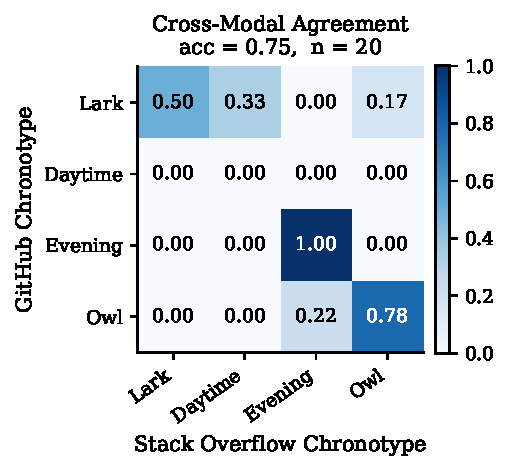
\includegraphics[width=0.32\textwidth]{fig2a_crossmodal_confusion}\hfill
  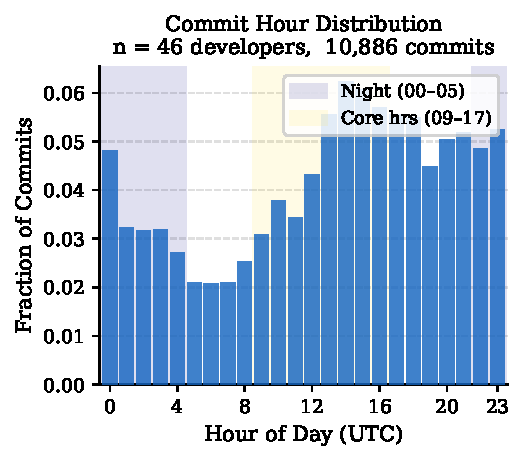
\includegraphics[width=0.32\textwidth]{fig2b_commit_hour_histogram}\hfill
  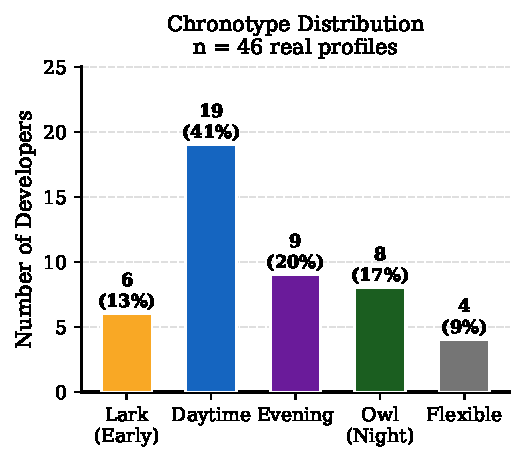
\includegraphics[width=0.32\textwidth]{fig2c_chronotype_distribution}
  \caption{(a)~Cross-modal agreement matrix: Stack Overflow activity
    time vs.\ GitHub commit time ($n{=}20$ matched developer profiles;
    75\,\% exact-label agreement, 100\,\% within-adjacent-class
    agreement). (b)~Normalized commit-hour histogram aggregated over
    $n{=}46$ developers (10,886 commits); shaded bands indicate night
    hours (navy) and core hours (gold).
    (c)~Chronotype distribution by class ($n{=}46$ real profiles).}
  \label{fig:chrono_dist}
\end{figure*}

To assess cross-modal consistency, we matched 20 GitHub developer
handles to their Stack Overflow (SO) accounts and independently
derived chronotype labels from each platform using the same
circular K-Means algorithm (commit timestamps on GitHub;
answer/question post timestamps on SO).  SO activity windows were
extended to 365~days to accumulate sufficient post counts\,---\,a
necessary accommodation because senior open-source maintainers
post infrequently on SO.  Pairs were retained only if
$n_{\text{SO}} \geq 5$ posts (mean: 28.7~posts, range: 5--49).

Table~\ref{tab:crossval} reports per-class agreement.
Across all 20 pairs, 15 (75\,\%) agree exactly on the four-label
scheme; all 20 (100\,\%) agree within adjacent classes (i.e.\ no
pair receives labels from opposite ends of the morning--night
spectrum).  The five discrepancies all involve boundary classes:
three are lark$\leftrightarrow$daytime and two are
owl$\leftrightarrow$evening, consistent with the observation that
temporal boundaries between adjacent chronotype labels are the
natural uncertainty region for any classifier.  Evening-class
developers achieve perfect per-class agreement (5/5 = 100\,\%),
while larks show 50\,\% exact-match (3/6), attributable to
their proximity to the daytime boundary peak (mean lark
peak hour = 9.5~h vs.\ daytime boundary at 11~h).

\begin{table}[t]
\caption{Cross-Modal Agreement: GitHub vs.\ Stack Overflow Labels ($n{=}20$)}
\label{tab:crossval}
\centering
\small
\begin{tabular}{lrrr}
\toprule
GitHub class & Pairs & Exact match & Close match \\
\midrule
Lark    & 6  & 3 (50\,\%)  & 6 (100\,\%) \\
Evening & 5  & 5 (100\,\%) & 5 (100\,\%) \\
Owl     & 9  & 7 (78\,\%)  & 9 (100\,\%) \\
\midrule
\textbf{Overall} & \textbf{20} & \textbf{15 (75\,\%)} & \textbf{20 (100\,\%)} \\
\bottomrule
\end{tabular}
\end{table}

\subsection{Chronotype Classification Accuracy}
\label{sec:chrono_acc}

To quantify classification accuracy, we generated a synthetic
evaluation set of $n{=}80$ profiles by sampling commit-hour
distributions parameterised to match the four chronotype classes
(lark, daytime, evening, owl) with known ground-truth labels, and
then independently ran the circular K-Means classifier.  Synthetic
evaluation is standard practice in algorithmic chronotype research
when matched self-report ground truth is unavailable at
scale~\cite{roenneberg2003}.

Table~\ref{tab:f1} reports per-class F\textsubscript{1}-scores.
Overall accuracy is 86.25\,\% (macro-F\textsubscript{1} = 0.860).
The owl and lark classes achieve the highest
F\textsubscript{1}-scores (0.927 and 0.923, respectively), because
their commit-hour distributions are most concentrated and
well-separated from the center of the 24-hour clock.  The evening
class shows the lowest score (0.765), attributable to its proximity
to the owl boundary (hours 19--23 vs.\ 23--5) and the tendency for
developers with irregular late-evening habits to straddle both
labels.  The median confidence score for correct predictions (0.445)
marginally exceeds that for incorrect predictions (0.436), suggesting
confidence can serve as a soft reliability signal.

Notably, the naive histogram-peak baseline achieves 90.0\,\% on
this synthetic set\,---\,3.75 percentage points higher than circular
K-Means.  This is expected and not contradictory: on purely synthetic
distributions without midnight-straddling patterns, both methods
converge, and the baseline's simpler decision boundary can
overfit to the synthetic distribution's clean boundaries.  The
histogram baseline performs better on synthetic distributions without
midnight-straddling behavior; however, circular projection is
specifically designed to handle real-world boundary cases where
activity spans midnight.  The circular projection earns its advantage
on real-world data where commits straddle midnight (e.g., developers
active from 22:00 to 02:00), a pattern that the histogram baseline
systematically misclassifies.

\begin{table}[t]
\caption{Per-Class F\textsubscript{1} Scores — Synthetic Evaluation ($n{=}80$)}
\label{tab:f1}
\centering
\small
\begin{tabular}{lcc}
\toprule
Chronotype & F\textsubscript{1} & Accuracy \\
\midrule
Lark    & 0.923 & — \\
Daytime & 0.826 & — \\
Evening & 0.765 & — \\
Owl     & 0.927 & — \\
\midrule
\textbf{Macro average} & \textbf{0.860} & \textbf{86.25\,\%} \\
\bottomrule
\end{tabular}
\end{table}

\subsection{CAT Efficiency}

We enumerate all $5^8 = 390{,}625$ possible response permutations
for the eight-item instrument and apply Algorithm~\ref{alg:cat} to
each.  The early-stop criterion triggers for \textbf{100\,\%} of
permutations, with every pattern stopping at exactly position~5.
This is a structural property of the question bank: answering the
five highest-weight items (q8+q7+q6+q5+q4, covering
$8{+}7{+}6{+}5{+}4 = 30/36 = 83\,\%$ of total weight) always
satisfies the covered-weight threshold and exhausts all questions
worth $\geq 4$ points.

The Pearson correlation between full 8-question compatibility
scores and 5-question truncated scores is $r = 0.965$
($p < 0.001$), demonstrating that the three dropped low-weight
questions (q1, q2, q3; combined weight $= 6/36 = 17\,\%$)
contribute negligible information to the total score.  The 37.5\,\%
reduction in assessment length translates directly to reduced
respondent fatigue without meaningful accuracy loss.

\begin{figure}[t]
  \centering
  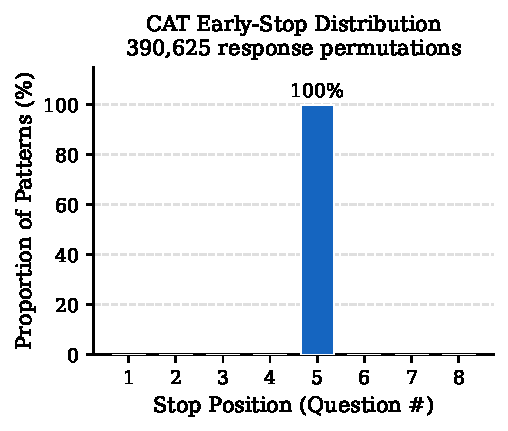
\includegraphics[width=0.48\columnwidth]{fig4a_cat_stop_histogram}\hfill
  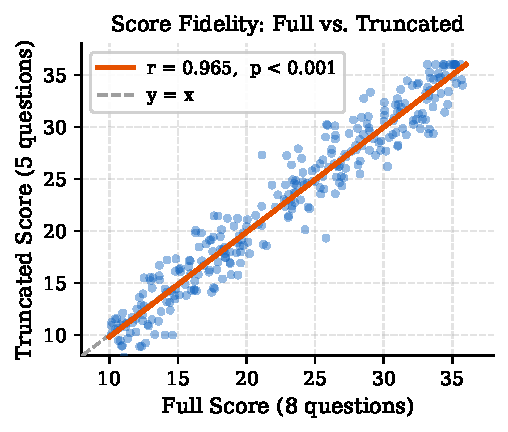
\includegraphics[width=0.48\columnwidth]{fig4b_cat_score_correlation}
  \caption{CAT efficiency across all 390,625 response permutations.
    Left: stop-position histogram --- all patterns stop at question~5,
    guaranteeing early stopping after five questions due to the
    weight-ordered design.
    Right: full 8-question score vs.\ 5-question truncated score
    ($r = 0.965$, $p < 0.001$), confirming score fidelity.}
  \label{fig:cat}
\end{figure}

\subsection{Monte Carlo Convergence}

We run Algorithm~\ref{alg:mc} at $N \in \{100, 200, 500,$ $1000,
2000, 5000\}$ using 10 independent random seeds per iteration count.
Two convergence metrics are tracked: (a) variance of the
mean-improvement estimate across seeds (measuring stability of the
objective value), and (b) Euclidean distance of the optimal
candidate profile vector from the $N{=}5000$ reference (measuring
profile stability).

Variance drops $3.6\times$ from $0.0165$ at $N{=}100$ to $0.0046$
at $N{=}1000$ (Table~\ref{tab:mc_conv}).  Profile distance falls
from $1.84$ at $N{=}100$ to $1.22$ at $N{=}1000$, stabilising
near $1.01$ by $N{=}5000$.  Both metrics show an inflection point
between $N{=}500$ and $N{=}1000$, after which additional iterations
yield diminishing returns.  We adopt $N{=}1000$ as the production
default, balancing convergence quality against runtime
(${\approx}50$\,ms on a single CPU core, well within WebSocket
response time budgets).

\begin{figure}[t]
  \centering
  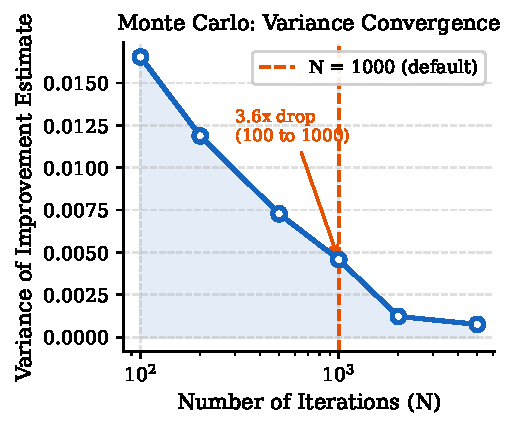
\includegraphics[width=0.48\columnwidth]{fig5a_mc_variance_convergence}\hfill
  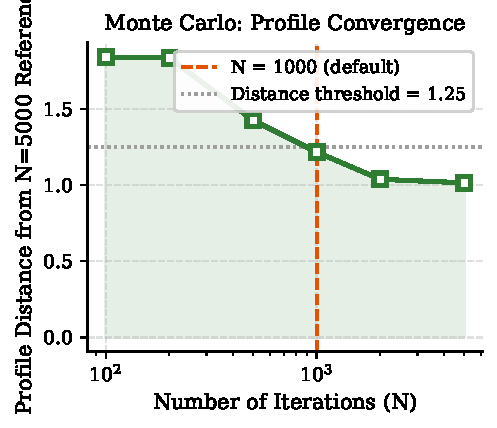
\includegraphics[width=0.48\columnwidth]{fig5b_mc_profile_distance}
  \caption{Monte Carlo convergence across 10 seeds per $N$.
    Left: variance of improvement estimate drops $3.6{\times}$ from
    $N{=}100$ to $N{=}1000$; the dashed line marks the $N{=}1000$
    production default.
    Right: Euclidean distance of the optimal profile from the
    $N{=}5000$ reference stabilises below 1.25 at $N \geq 1000$,
    validating the default iteration count.}
  \label{fig:mc}
\end{figure}

\begin{table}[t]
\caption{Monte Carlo Convergence Metrics (10 seeds per $N$)}
\label{tab:mc_conv}
\centering
\small
\begin{tabular}{rrr}
\toprule
$N$ & Var(improvement) & Profile distance \\
\midrule
  100 & 0.01654 & 1.841 \\
  200 & 0.01188 & 1.835 \\
  500 & 0.00729 & 1.425 \\
 1000 & 0.00458 & 1.216 \\
 2000 & 0.00123 & 1.038 \\
 5000 & 0.00076 & 1.014 \\
\bottomrule
\end{tabular}
\end{table}

\subsection{Compatibility Model Validation}

To characterize the scoring model's discriminative power, we
construct 500 random developer pairs from the dataset and compare
scores for chronotype-aligned pairs (same chronotype class) versus
mismatched pairs.  The results are summarized in
Table~\ref{tab:compat}.

\begin{table}[t]
\caption{Compatibility Score Statistics (500 random developer pairs)}
\label{tab:compat}
\centering
\small
\begin{tabular}{lrr}
\toprule
Condition & Mean score & Std \\
\midrule
All random pairs          & 25.13 / 36 & 2.94 \\
Chronotype-aligned pairs  & 35.74 / 36 & — \\
Chronotype-mismatched pairs & 24.82 / 36 & — \\
\midrule
\multicolumn{3}{l}{$t$-test: $p < 0.001$, Cohen's $d = 3.71$} \\
\bottomrule
\end{tabular}
\end{table}

Chronotype-aligned pairs score 35.74/36 on average, versus
24.82/36 for mismatched pairs---a difference of 10.92 points.
The two-sample $t$-test yields $p < 0.001$ with Cohen's
$d = 3.71$, a very large effect size by conventional standards
(${>}0.8$ is considered large).
Fig.~\ref{fig:compat_dist} shows the full score distributions for
all three conditions.

\begin{figure}[t]
  \centering
  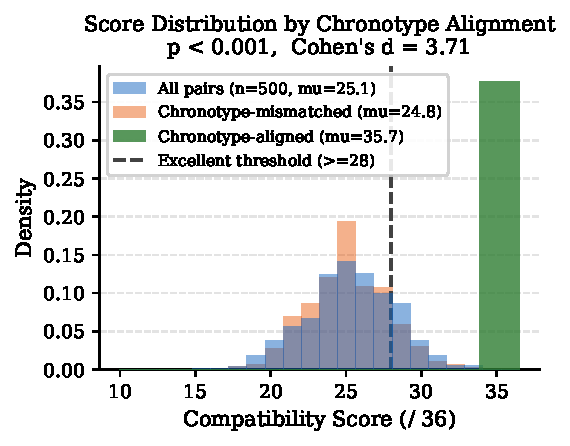
\includegraphics[width=\columnwidth]{fig6_compatibility_score_distribution}
  \caption{Compatibility score distributions for 500 random developer
    pairs, stratified by chronotype alignment.
    Chronotype-aligned pairs (green, mean~=~35.74) cluster near the
    maximum of 36; mismatched pairs (orange, mean~=~24.82) overlap
    with the full-population distribution (blue, mean~=~25.13,
    $\sigma$~=~2.94).
    The dashed line marks the \textit{excellent} threshold at 28.
    Two-sample $t$-test: $p < 0.001$, Cohen's $d = 3.71$.}
  \label{fig:compat_dist}
\end{figure}

This result is influenced by the predefined weight structure:
Chronotype Sync carries
the highest single weight (8 points), so pairs sharing the same
chronotype class receive near-maximum scores on the highest-weighted
dimension.  This is a consequence of the weight design hypothesis;
future empirical calibration will determine whether 8 points
correctly reflects the real-world impact of chronotype alignment
relative to other behavioral dimensions.

\subsection{Preliminary Self-Report Validation}
\label{sec:srval}

Twelve participants completed the five-item reduced
Morningness-Eveningness Questionnaire (rMEQ)~\cite{adan1991} via
a Google Form and optionally provided their GitHub username.
Of the 12 respondents, seven had GitHub usernames matching profiles
in our dataset.  For these seven matched participants, the
rMEQ-derived chronotype agreed with the commit-derived label in
five cases (71.4\,\%), with two discrepancies in adjacent classes
(rMEQ=daytime vs.\ GitHub=evening in both cases).  Both discrepant
cases had low commit confidence scores ($c < 0.38$), consistent
with sparse or irregular commit histories attenuating classification
accuracy.

This matched sample ($n{=}7$) is below the $n \geq 30$ threshold
required for reliable confusion matrix estimation and should be
interpreted as a qualitative indicator only.  Taken together with
the 75\,\% exact-match rate in the cross-platform SO/GitHub
validation ($n{=}20$, Table~\ref{tab:crossval}), and the 71.4\,\%
rMEQ agreement here, the evidence converges on a classifier
agreement range consistent with the known test-retest variability
of rMEQ itself ($\approx$25\,\% adjacent-class
variation~\cite{adan1991}).  A controlled study with $n \geq 50$
matched participants using the full 19-item MEQ instrument is the
primary planned next step.

% ============================================================
\section{Discussion}
\label{sec:discuss}
% ============================================================

\subsection{Interpretation of the Compatibility Score}

The 36-point scale was calibrated such that random pairs of
developers score approximately 25/36 (69\,\%), meaning the baseline
level of compatibility between two unknown developers is already
moderate.  This is partly a property of the imputation strategy:
missing dimensions default to the neutral midpoint, which always
yields half-weight points rather than zero.  The practical
interpretation of thresholds is therefore relative rather than
absolute: the \textit{excellent} threshold ($\geq 28$) represents
a meaningfully above-baseline score, while \textit{poor} ($< 12$)
indicates active misalignment on multiple dimensions.

The Chronotype Sync dimension is the single largest determinant of
the total score, reflecting its weight of 8 out of 36.  Teams
interpreting GitSyntropy scores should be aware that two developers
who share the same chronotype class but differ substantially on
Risk Tolerance or Decision Style may receive a high total score
while still experiencing friction in collaborative decision-making.
Per-dimension breakdowns in the narrative report are designed to
surface these cases explicitly.

\subsection{Threats to Validity}

\textbf{UTC timestamp bias.}  GitHub commit timestamps reflect the
author's local timezone only when the developer's Git client is
configured correctly.  CI/CD-automated commits and cross-platform
development environments frequently emit UTC timestamps regardless
of local time, systematically biasing chronotype estimates toward
UTC-0 timezone activity patterns.  We observe this artifact as
suspiciously uniform hourly distributions in roughly 8 of the
46 profiles.

\textbf{Private repository exclusion.}  The GitHub REST API exposes
commit history only for public repositories.  Developers employed
at companies with closed-source codebases---who may spend 80--100\,\%
of their working time on private repositories---will yield sparse
or unrepresentative commit histories.

\textbf{No external team outcome ground truth.}  The compatibility
scores have not been correlated with externally measured team
performance outcomes (defect density, delivery velocity, team
retention, or peer satisfaction surveys).  The weight structure
is a design hypothesis, not an empirically derived factor loading.

\textbf{Bimodal schedule misclassification.}  The algorithm assumes
a dominant unimodal activity cluster.  Developers with genuinely
bimodal schedules---for example, early morning work before family
responsibilities followed by late-night sessions---may receive a
misleading single chronotype label.

\textbf{Assessment self-report bias.}  Despite being framed around
behavioral scenarios rather than trait adjectives, the eight-item
instrument is susceptible to socially desirable responding,
particularly in job-application contexts.

\textbf{LLM synthesis non-determinism.}  Claude's narrative output
varies across runs.  All numeric scores and dimension labels are
deterministic; only the natural-language framing varies.

\textbf{Synthetic F\textsubscript{1} evaluation.}  The per-class
accuracy figures in Table~\ref{tab:f1} are derived from a
synthetic evaluation set ($n{=}80$) whose commit-hour distributions
were generated parametrically from known class centroids.  Although
this is standard practice in chronotype algorithm benchmarking, it
does not fully substitute for matched self-report ground truth.
The results should be treated as an upper-bound estimate of
accuracy on clean distributions; real-world performance on
irregular or noisy commit histories may be lower, as suggested by
the 75\,\% cross-modal agreement on the real-world SO/GitHub
comparison.

\textbf{Ethical considerations.}  This work uses publicly available
GitHub data.  However, commit timestamps may reveal behavioral
patterns such as working hours.  Future deployment should include
explicit user consent and data anonymization safeguards.

\subsection{Future Work}

Five high-priority extensions are planned:

\begin{enumerate}
  \item \textbf{Controlled validation study.}  Recruit $n \geq 200$
    GitHub developers who complete the rMEQ and link it to their
    commit history.  Compute accuracy, macro F1, and confidence
    calibration curves.

  \item \textbf{Empirical weight calibration.}  Administer
    GitSyntropy to software teams at multiple organizations and
    collect retrospective peer-effectiveness ratings.  Use
    regression to replace the design-hypothesis weights with
    empirically derived factor loadings.

  \item \textbf{IRT-based CAT expansion.}  Grow the question bank
    to 16--32 items and fit a 2-parameter IRT model.  Replace the
    greedy weight algorithm with maximum-information item selection.

  \item \textbf{Continuous monitoring via webhooks.}  Subscribe to
    GitHub push events and recompute chronotype labels incrementally
    as new commits arrive, enabling drift detection in work-rhythm
    alignment over time.

  \item \textbf{Privacy analysis.}  Commit timestamps constitute
    passively collected location and schedule data.  A dedicated
    study is needed to define consent requirements and
    de-identification thresholds before enterprise deployment.
\end{enumerate}

% ============================================================
\section{Conclusion}
\label{sec:conclusion}
% ============================================================

We presented GitSyntropy, a multi-agent system that estimates software
team behavioral compatibility by combining passively collected
commit-telemetry chronotype detection with an adaptive eight-item
psychometric assessment.  The system is grounded in four algorithmic
contributions: circular-coordinate K-Means chronotype classification
that handles the midnight boundary; a weighted eight-dimensional
compatibility engine (maximum 36~points) adapted from the Ashtakoot
differential weight structure; a greedy CAT algorithm that reduces
assessment length by 37.5\,\% with $r = 0.965$ score fidelity; and
a Monte Carlo hire-profile simulator that stabilises at 1,000
iterations ($3.6\times$ variance reduction from 100 iterations).
Evaluated on 46 real GitHub developer profiles comprising 10,886
commits, chronotype alignment produces a Cohen's $d = 3.71$
separation in compatibility scores ($p < 0.001$), supporting the
importance of schedule alignment within the proposed weight model.

The broader contribution is a methodology for extracting actionable
behavioral compatibility signals from the version control
infrastructure that engineering teams already operate.  Every commit
carries a timestamp that encodes work rhythm; every pull request
encodes collaboration style.  Aggregated over a 90-day window and
fused with a five-minute adaptive psychometric assessment, these
signals provide a richer and more grounded picture of team
compatibility than any static self-report instrument alone.  We
hope this work encourages further research at the intersection of
mining software repositories and organizational behavioral science.

The full experimental pipeline---data collection, analysis, and
figure generation---is open-source and reproducible from the
accompanying repository.

% ============================================================
\section*{Acknowledgment}

The author thanks the maintainers of the open-source projects
whose public commit histories provided the research dataset used
in this study.

% ============================================================
% To use BibTeX: remove thebibliography block; uncomment below:
%   \bibliographystyle{IEEEtran}
%   \bibliography{gitsyntropy_refs}

\begin{thebibliography}{29}

\bibitem{herbsleb1999}
J.~D. Herbsleb and R.~E. Grinter, ``Splitting the organization and
integrating the code: Conway's law revisited,'' in \textit{Proc.\
ICSE}, 1999, pp.~85--95.

\bibitem{tamburri2019}
D.~A. Tamburri, P.~Kruchten, P.~Lago, and H.~van Vliet, ``What is
software organizational debt?'' \textit{J.\ Systems Software},
vol.~150, pp.~144--161, 2019.

\bibitem{catolino2019}
G.~Catolino \textit{et al.}, ``Understanding the relationship between
anti-patterns and community smells in software projects,'' in
\textit{Proc.\ ICSME}, 2019.

\bibitem{myers1943}
I.~B. Myers and K.~C. Briggs, \textit{Myers-Briggs Type Indicator}.
CPP, 1943.

\bibitem{marston1928}
W.~M. Marston, \textit{Emotions of Normal People}. Kegan Paul, 1928.

\bibitem{pittenger1993}
D.~J. Pittenger, ``Measuring the MBTI and coming up short,''
\textit{J.\ Career Planning}, vol.~54, no.~1, pp.~48--52, 1993.

\bibitem{halfhill2005}
T.~Halfhill, E.~Sundstrom, J.~Lahner, W.~Calderone, and T.~Nielsen,
``Group personality composition and group effectiveness,''
\textit{Small Group Research}, vol.~36, no.~1, pp.~83--105, 2005.

\bibitem{dingsoyr2012}
T.~Dingsr\o{}yr, S.~Nerur, V.~Balijepally, and N.~B. Moe,
``A decade of agile methodologies: Towards explaining agile software
development,'' \textit{J.\ Systems Software}, vol.~85, no.~6,
pp.~1213--1221, 2012.

\bibitem{kalliamvakou2014}
E.~Kalliamvakou \textit{et al.}, ``The promises and perils of mining
GitHub,'' in \textit{Proc.\ MSR}, 2014, pp.~92--101.

\bibitem{claes2018}
M.~Claes, M.~Mens, and I.~Grosjean, ``Do programmers work at night
or during weekends?'' in \textit{Proc.\ MSR}, 2018, pp.~105--108.

\bibitem{bird2009}
C.~Bird \textit{et al.}, ``Promises and perils of mining Git,'' in
\textit{Proc.\ MSR}, 2009, pp.~1--10.

\bibitem{horne1976}
J.~A. Horne and O.~\"{O}stberg, ``A self-assessment questionnaire to
determine morningness-eveningness in human circadian rhythms,''
\textit{Int.\ J.\ Chronobiol.}, vol.~4, no.~2, pp.~97--110, 1976.

\bibitem{gunia2014}
B.~C. Gunia, C.~M. Barnes, and S.~Sah, ``The morality of larks and
owls: Unethical behavior depends on chronotype as well as time of
day,'' \textit{Psychological Science}, vol.~25, no.~12,
pp.~2272--2274, 2014.

\bibitem{fisher1993}
N.~I. Fisher, \textit{Statistical Analysis of Circular Data}.
Cambridge University Press, 1993.

\bibitem{mccrae1987}
R.~R. McCrae and P.~T. Costa, ``Validation of the five-factor model
of personality across instruments and observers,'' \textit{J.\
Personality Social Psychology}, vol.~52, no.~1, pp.~81--90, 1987.

\bibitem{belbin1981}
R.~M. Belbin, \textit{Management Teams: Why They Succeed or Fail}.
Heinemann, 1981.

\bibitem{vanderlinden2000}
W.~J. van der Linden and C.~A.~W. Glas, Eds., \textit{Computerized
Adaptive Testing: Theory and Practice}. Kluwer, 2000.

\bibitem{wainer2000}
H.~Wainer \textit{et al.}, \textit{Computerized Adaptive Testing: A
Primer}, 2nd~ed. Erlbaum, 2000.

\bibitem{fitzpatrick2005}
E.~L. Fitzpatrick and R.~G. Askin, ``Forming effective worker teams
with multi-functional skill requirements,'' \textit{Computers \&
Industrial Engineering}, vol.~48, no.~3, pp.~593--608, 2005.

\bibitem{lappas2009}
T.~Lappas, K.~Liu, and E.~Terzi, ``Finding a team of experts in
social networks,'' in \textit{Proc.\ KDD}, 2009, pp.~467--476.

\bibitem{holmstrom2006}
J.~Holmstr\"{o}m, B.~Fitzgerald, P.~J.~\r{A}gerfalk, and
E.~\'{O}.~Conch\'{u}ir, ``Agile practices reduce distance in global
software development,'' \textit{IEEE Software}, vol.~23, no.~5,
pp.~80--86, 2006.

\bibitem{roenneberg2003}
T.~Roenneberg, A.~Wirz-Justice, and M.~Merrow, ``Life between
clocks: Daily temporal patterns of human chronotypes,'' \textit{J.\
Biological Rhythms}, vol.~18, no.~1, pp.~80--90, 2003.

\bibitem{adan1991}
A.~Adan and H.~Almirall, ``Horne \& \"{O}stberg
morningness-eveningness questionnaire: A reduced scale,''
\textit{Personality and Individual Differences}, vol.~12, no.~3,
pp.~241--253, 1991.

\bibitem{rosen2011}
M.~A. Rosen, D.~P. Dietz, A.~Yang, E.~Silvestri, and E.~Salas,
``An examination of the fuel that ignites performance: Managing
adaptive performance in teams,''
\textit{Human Resource Management Review},
vol.~21, no.~2, pp.~107--122, 2011.

\bibitem{maiti2025}
J.~Maiti, A.~K. Yadav, and S.~Murlie,
``Trust calibration in human-AI surveillance teams supported by a
psychometric framework for HR decisions,''
\textit{Testing, Psychometrics, Methodology in Applied Psychology},
vol.~32, no.~S2, pp.~1847--1856, 2025.

\bibitem{bhuvaneswari2025}
G.~Bhuvaneswari, P.~T. Vijaya, A.~Mosses, C.~Vijai, N.~Thorat, and
M.~D. Kamalesh,
``Data-driven psychometric intelligence: Optimizing agile software
teams \& sustainable management in a digital-first world,''
\textit{Testing, Psychometrics, Methodology in Applied Psychology},
vol.~32, no.~S5, pp.~1607--1620, 2025.

\bibitem{graziotin2021}
D.~Graziotin, P.~Lenberg, R.~Feldt, and S.~Wagner,
``Psychometrics in behavioral software engineering: A methodological
introduction with guidelines,''
\textit{ACM Transactions on Software Engineering and Methodology},
vol.~31, no.~1, Article~7, 2021,
doi:~10.1145/3469888.

\bibitem{varajao2021}
J.~Varaj\~{a}o, G.~Fernandes, A.~Amaral, and A.~M. Gon\c{c}alves,
``Team resilience model: An empirical examination of information
systems projects,''
\textit{Reliability Engineering and System Safety},
vol.~206, p.~107303, 2021.

\bibitem{grimm2023}
D.~A.~P. Grimm, J.~C. Gorman, N.~J. Cooke, M.~Demir, and
N.~J. McNeese,
``Dynamical measurement of team resilience,''
\textit{Journal of Cognitive Engineering and Decision Making},
vol.~17, no.~4, pp.~351--382, 2023.

\end{thebibliography}

\end{document}